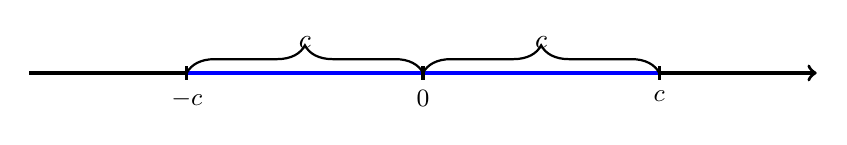
\begin{tikzpicture}
  \coordinate (A) at (-5,0);
  \coordinate (B) at (5,0);
  
  \coordinate (C) at (3,0);
  \coordinate (-C) at (-3,0);
  \coordinate (O) at (0,0);
  
  \draw [very thick,\lt->] (A) -- (B);
  \draw [very thick,blue] (-C) -- (C);
  
  \draw [very thick] (-3,2.5pt) -- +(0,-5pt) node [anchor=north, font=\small] {$-c$};
  \draw [very thick] (0,2.5pt) -- +(0,-5pt) node [anchor=north, font=\small] {$0$};
  \draw [very thick] (3,2.5pt) -- +(0,-5pt) node [anchor=north, font=\small] {$c$};

  \draw[thick,decorate,decoration={brace,amplitude=10pt},yshift=2.5pt] (-C) -- (O) node [midway,above,yshift=5pt] {$\abs{c}$};
  \draw[thick,decorate,decoration={brace,amplitude=10pt},yshift=2.5pt] (O) -- (C) node [midway,above,yshift=5pt] {$\abs{c}$};
\end{tikzpicture}
